\section{Разработка программного обеспечения на C\#}

\subsection{Полный код программы}

Ниже представлен полный листинг программы на языке C\#.

\begin{minted}{cs}
using System;

namespace ElectricCircuitCalculator
{
    class Program
    {
        static void Main()
        {
            Console.Title = "Расчёт электрической цепи";
            Console.WriteLine("РАСЧЁТ ЦЕПИ ПОСТОЯННОГО ТОКА\n");

            Console.Write("Напряжение U (В): ");
            double U = double.Parse(Console.ReadLine());
            Console.Write("R1 (Ом): ");
            double R1 = double.Parse(Console.ReadLine());
            Console.Write("R2 (Ом): ");
            double R2 = double.Parse(Console.ReadLine());
            Console.Write("R3 (Ом): ");
            double R3 = double.Parse(Console.ReadLine());

            // Проверка корректности ввода
            if (U <= 0 || R1 <= 0 || R2 <= 0 || R3 <= 0)
            {
                Console.WriteLine("Ошибка: все значения должны 
                быть положительными!");
                return;
            }

            // Расчёт по формулам
            // 1. Эквивалентное сопротивление параллельного участка
            double R23 = (R2 * R3) / (R2 + R3);
            
            // 2. Общее сопротивление цепи
            double R_total = R1 + R23;
            
            // 3. Общий ток цепи (закон Ома)
            double I_total = U / R_total;
            
            // 4. Токи и напряжения на элементах
            double I1 = I_total;
            double U1 = I1 * R1;
            double U23 = U - U1;
            double I2 = U23 / R2;
            double I3 = U23 / R3;
            
            // 5. Мощности
            double P1 = I1 * I1 * R1;
            double P2 = I2 * I2 * R2;
            double P3 = I3 * I3 * R3;
            double P_source = U * I_total;
            double P_load = P1 + P2 + P3;
            
            // 6. Погрешность баланса мощностей
            double error = Math.Abs(P_source - P_load) / P_source * 100;

            Console.WriteLine("Элемент   R(Ом)    I(А)     U(В)     P(Вт)");
            
            Console.WriteLine($"R1        {R1,6:F2} {I1,6:F3} {U1,6:F2} {P1,6:F2}");
            Console.WriteLine($"R2        {R2,6:F2} {I2,6:F3} {U23,6:F2} {P2,6:F2}");
            Console.WriteLine($"R3        {R3,6:F2} {I3,6:F3} {U23,6:F2} {P3,6:F2}");
            Console.WriteLine($"Источник  {'-',6} {I_total,6:F3} {U,6:F2} {P_source,6:F2}");
            
            Console.WriteLine("\nНажмите любую клавишу...");
            Console.ReadKey();
        }
    }
}
\end{minted}

\subsection{Результат работы программы}

На рисунке \ref {img:pic2} представлен результат выполнения программы для исходных данных U = 100 В, R1 = 100 Ом, R2 = 200 Ом, R3 = 300 Ом.

\begin{figure}[H]
    \centering
    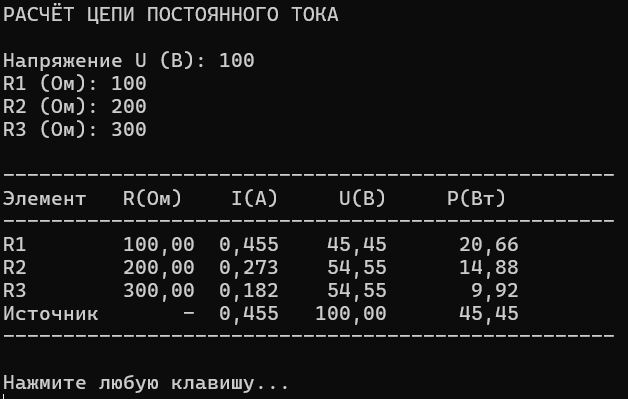
\includegraphics[width=\textwidth]{pic2.png}
    \caption{Сравнение полученных результатов}
    \label{img:pic2}
\end{figure} 
